\section{Hierarchical triple star systems}\label{sec:triples_evolution}

The majority triple star systems are observed in hierarchical structures. More specifically, they consist of an inner binary and a distant star (hereafter tertiary/outer star) that orbits the center of mass of the inner binary system such as $\frac{\alpha_{in}}{\alpha_{out}} << 1$. A schematic of a hierarchical triple system is presented in \cref{fig:triple_schem}.
\begin{figure}[H]
    \centering
    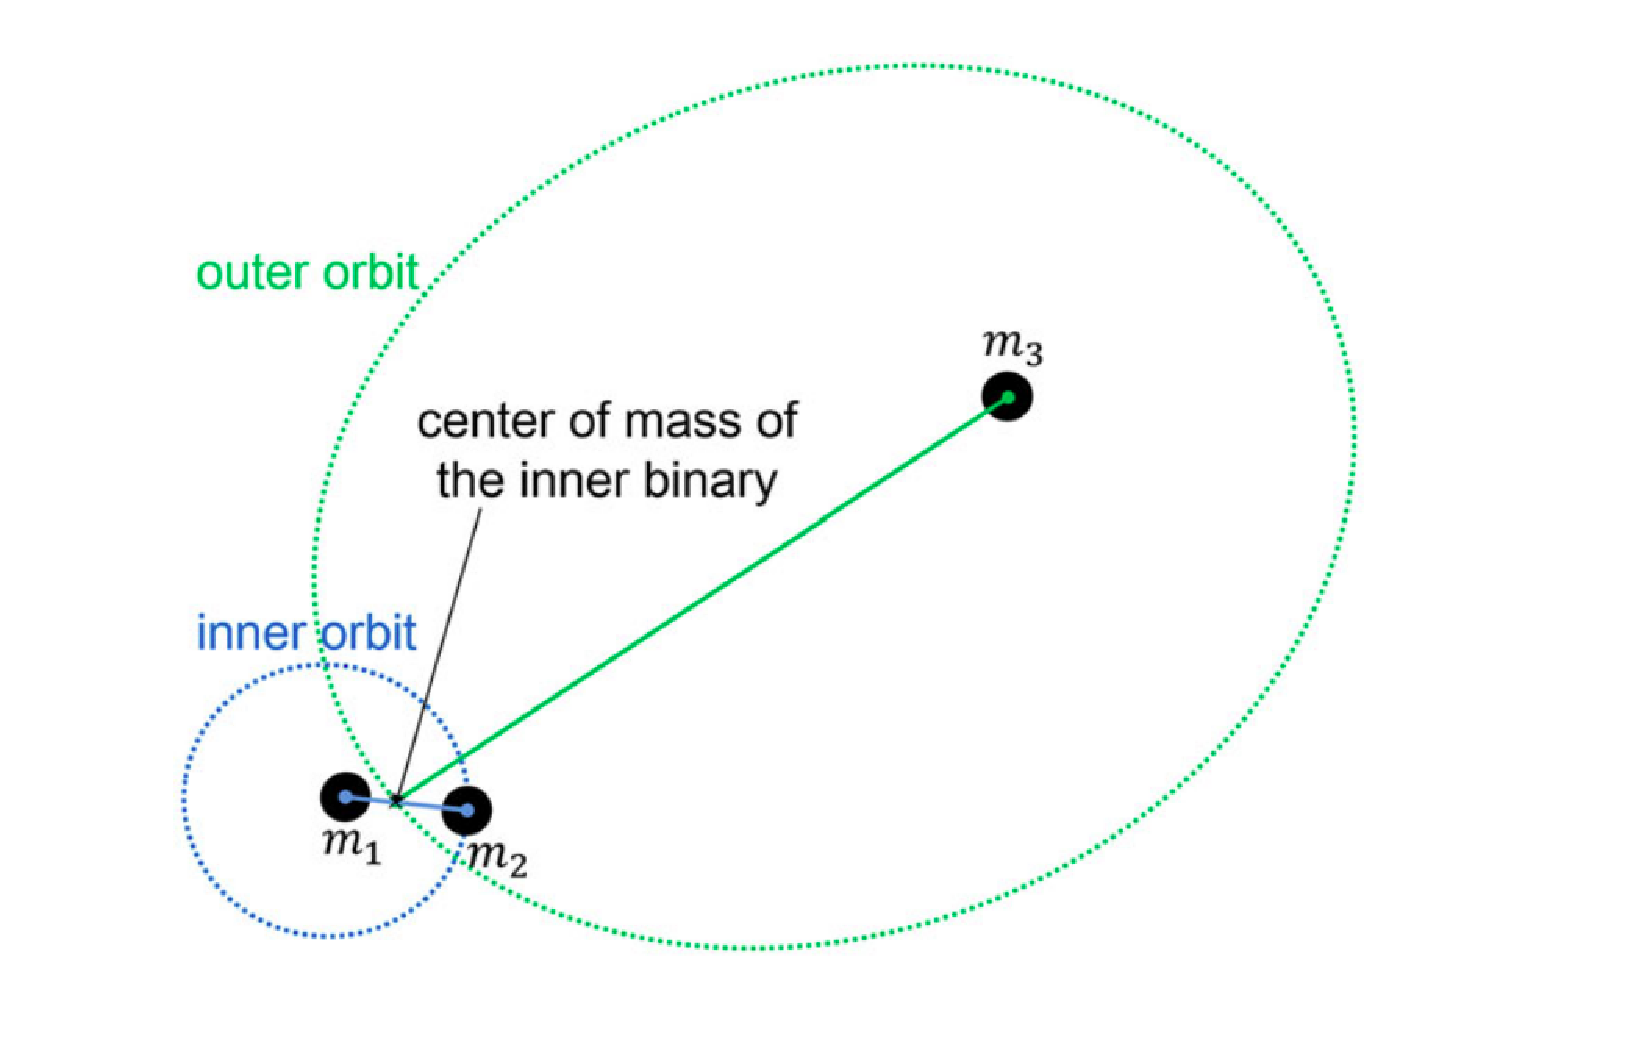
\includegraphics[width=0.9\textwidth]{Thesis/figures/triple_schem.pdf}
    \caption{A schematic of a hierarchical triple system consisting of an inner and an outer binary. The inner binary consists of objects whose masses are $m_1$ and $m_2$, and the outer one is the pair of the inner binary and the third body with mass $m_3$. Figure taken by \cite{gupta2020gravitational}.}
    \label{fig:triple_schem}
\end{figure}
In certain situations, the presence of the outer star does not alter the evolution of the inner binary. In such cases, the evolution of the tertiary  and the inner binary can be studied separately. In other circumstances, the three stars interact in ways that are unique to systems with multiplicities higher than binaries. As a result, numerous new evolutionary paths are anticipated compared to binary evolution. In the following subections, I focus on the dynamical stability of triple systems and the Lidov-Kozai cycles. These topics are relevant to my work, but for a detailed overview of triple evolution I direct the reader to \cite{michaely2014secular,toonen2016evolution}.

\subsection{Stability of triples}\label{sub:stability_triples}

Unlike two-body systems, the three-body problem does not have closed-form solutions. On the one hand, triple systems in the unstable regime tend to disintegrate into lower order systems on dynamical timescales \citep{van2007formation}. On the other hand, stability can occur (and last) on different timescales, thus it is not trivial to draw a clear line between stable and unstable triple systems. 

\cite{mardling1999dynamics} stability criterion is usually used in studies of triple systems' evolution, where a system is unstable if
$\frac{\alpha_{in}}{\alpha_{out}} < \frac{\alpha_{in}}{\alpha_{out}} |_{crit}$. The critical fraction is given as:
\begin{equation}\label{eq:stability_regime}
    \frac{\alpha_{in}}{\alpha_{out}} |_{crit} = \frac{2.8}{1-e_{out}} (1- \frac{0.3 i_{mut}}{\pi}) \left ( \frac{(1 + q_{out})(1+e_{out})}{\sqrt{1-e_{out}}} \right )^{2/5},
\end{equation}
where $q_{out} \equiv m_3 / (m_1 + m_2)$. The criterion is based on the concept of chaos and the result of overlapping resonances. The criterion is conservative since the existence of chaos is not always synonymous with instability. Many more stability criteria have been proposed and I direct the reader to \cite{mardling2001stability,georgakarakos2008stability}.

In \cref{sub:orbit_evol_mass_loss} I discussed how the orbital parameters change during non-conservative mass transfer. These concepts are also applicable for triples, where the orbital parameters of the inner and the outer orbit can change due to angular momentum loss from the system. As a result, initially stable triple systems can become dynamically unstable during their evolution.

\subsection{Lidov-Kozai cycles}\label{sub:lidov_kozai}

Dynamical interactions in hierarchical triples can differ from the case of binaries. The presence of the third star can give rise to the Lidov-Kozai mechanism \citep{lidov1962evolution,kozai1962secular}, which can have a significant impact on the secular evolution the system. During Lidov-Kozai cycles, the mutual torque between the inner and outer binary orbits result to angular momentum exchange. Furthermore, the orbital energy is preserved, and hence the semi-major axes are also conserved. Consequently, the orbital inner eccentricity and mutual inclination vary periodically (i.e. 'cycles'). When the inclination between the two orbits is minimized, the inner binary's eccentricity reaches its maximum. Furthermore, the pericenter argument may rotate or librate periodically.

Evolution during Lidov-Kozai cycles can be fairly complicated, but given some assumptions, analytical expressions can be derived. For example, in the test-particle approximation ($e_{in}=e_{out}=0$ and $M_2 << M_1, M_3$ \citep{naoz2013secular}), the mechanism is expected to take place only if $i_{mut} \in [39.2^{\circ},140.8^{\circ}$]. Furthermore, by expanding the three-body Hamiltonian to quadrupole order in $a_{in}/a_{out}$ \citep{kinoshita1999analytical}, the timescale for the Lidov-Kozai cycles is
\begin{equation}\label{eq:lidov_kozai_timescale}
    t_{kozai} \approx \frac{P_{out}^2}{P_{in}} + \frac{M_1 + M_2 +M_3}{M_3}(1-e_{out}^2)^{3/2},
\end{equation}
where $P_{in}$ and $P_{out}$ are the periods of the inner and outer orbit, respectively. Typically, $t_{kozai} >> P_{in},P_{out}$.

Higher orders of $a_{in}/a_{out}$, i.e. the octupole level of approximation, result to even richer dynamical behavior than the quadrupole approximation. The octupole term is expected to be important when $\epsilon_{oct} \geq 0.01$ \citep{naoz2011hot,shappee2013mass} and
\begin{equation}\label{eq:octupole_term}
    \epsilon_{oct} = \frac{M_1 - M_2}{M_1 + M_2} \frac{a_{in}}{a_{out}} \frac{e_{out}}{1-e_{out}^2}.
\end{equation}